\documentclass[conference]{IEEEtran}
\IEEEoverridecommandlockouts
% The preceding line is only needed to identify funding in the first footnote. If that is unneeded, please comment it out.
\usepackage{cite}
\usepackage{amsmath,amssymb,amsfonts}
\usepackage{algorithmic}
\usepackage{graphicx}
\usepackage{textcomp}
\usepackage{xcolor}
\def\BibTeX{{\rm B\kern-.05em{\sc i\kern-.025em b}\kern-.08em
    T\kern-.1667em\lower.7ex\hbox{E}\kern-.125emX}}

%\documentclass[conference,a4paper]{IEEEtran}					%导入IEEEtran的A4格式模板
%\usepackage[inner=0.9055in,outer=0.5118in,top=0.5in]{geometry}	%左边距inner,右边距outer,上边距top

\usepackage{amsmath}			%数学公式包
\allowdisplaybreaks[3] 			%导入数学公式包的前提下,允许跨页,1,2,3,4表示允许程度,但equation环境不可换页
								%长公式跨页可用align公式
\usepackage{bbm} 				%粗体、双线体
\usepackage{multirow} 			%纵向合并单元格
\usepackage{booktabs} 			%三线表
\usepackage{color}
\usepackage{amssymb}			%数学定理和证明过程包
\let\labelindent\relax
\usepackage{enumitem}			%调整垂直/水平间距/标签样式

\usepackage{amsthm}								%定理环境
\newtheorem{ownlemma}{Lemma} 					%引理。定理将两个lemma改为theorem 即可
\newtheorem{owncorollary}{Corollary}			%推论
\newtheorem{owndefinition}{Definition} 			%定义
\newtheorem{ownproperty}{Property} 				%性质

\usepackage{algorithm} 							%代码环境
\usepackage[noend]{algpseudocode}				%伪代码中 类似 if...end if去掉end if语句
\renewcommand{\algorithmicrequire}{Input:}
\renewcommand{\algorithmicensure}{Output:}
\renewcommand{\algorithmiccomment}[1]{// #1}	%C语言的注释格式

\bibliographystyle{IEEEtran}					%引用文献格式
\usepackage[numbers, sort & compress]{natbib} 	%压缩引用序号
\usepackage{hyperref}                           %引用链接
\usepackage{soul}   			%高亮显示,为提高本文可读性而添加,实际论文不需要该包

\begin{document}

%%%%%%%%% TITLE - PLEASE UPDATE
\title{FVHNet: Homography Matrix Estimation for Virtual Camera}
\author{Zhiming Hou, Yuanzhouhan Cao\textsuperscript{*}\thanks{\hrule \vspace{10pt} This work is supported by Beijing Natural Science Foundation (L221011). Yuanzhouhan Cao is the corresponding author.}}
%-------------------------------------------------------------------------
\maketitle

%%%%%%%%% ABSTRACT
\begin{abstract}
  Robust lane detection in real-time is one of the foundations for advanced autonomous driving,
which can provide substantial amounts of useful information for Autonomous Driving Systems (ADS), vehicle self-control, localization, and map construction.
Since the in/extrinsic parameters of different vehicles are various which has a significant impact on the results of 3D lanes,
we introduce the Virtual Camera that unifies the in/extrinsic parameters of cameras mounted on
different vehicles to guarantee the consistency of the spatial relationship among cameras.
It can effectively promote the learning procedure due to the unified visual space.
Different from the method of using fixed intrinsic parameters and extrinsic parameters to transformer front-view images to virtual images,
we train a network, termed HNet, that estimates the parameters of an ideal perspective transformation, conditioned on the input image.
In order to train FVHNet for outputting the transformation matrix that is optimal for perspective transformation, we construct a loss function referred FVHLoss.
In summary, we propose a model which can unify the in/extrinsic parameters of different vehicles.
We verify our method on the OpenLane dataset and achieve competitive results.
\end{abstract}
\begin{IEEEkeywords}
Homography, Virtual Camera, 3D Lane Detection.
\end{IEEEkeywords}
%%%%%%%%% INTRODUCTION
\section{Introduction}
\label{sec:intro}

As one of the foundation for safety in autonomous driving, many research efforts in lane detection focus on making detection model accurate and robust.
Over the past few years, 2D lane detection methods have shown impressive performances~\cite{jin2022eigenlanes, hou2019learning, liu2021end, wang2022keypoint, huang2023anchor3dlane}.
However, due to the lack of depth information, transforming 2D images to 3D space still remains highly challenging.
Recently, large-scale datasets with 3D lane annotations have been proposed.
This has been promoted the research of 3d lane line representation and detection~\cite{chen2022persformer, efrat20203d, garnett20193d, guo2020gen, liu2022learning, yan2022once, huang2023anchor3dlane}.
Compared to 2D lane, 3D lane detection can directly obtain the slope information of the lane, to help autonomous vehicles make better decisions.
%3D Lane Detection is critical for various applications in autonomous driving, such as trajectory planning and lane keeping.
%Despite the remarkable progress of LiDAR-based methods in other 3D perception tasks~\cite{zhou2018voxelnet, lang2019pointpillars},
%recent advances in 3D lane detection prefer using a monocular camera since it owns desirable advantages compared to LiDARs.


\begin{figure}[ht]
    \centering
    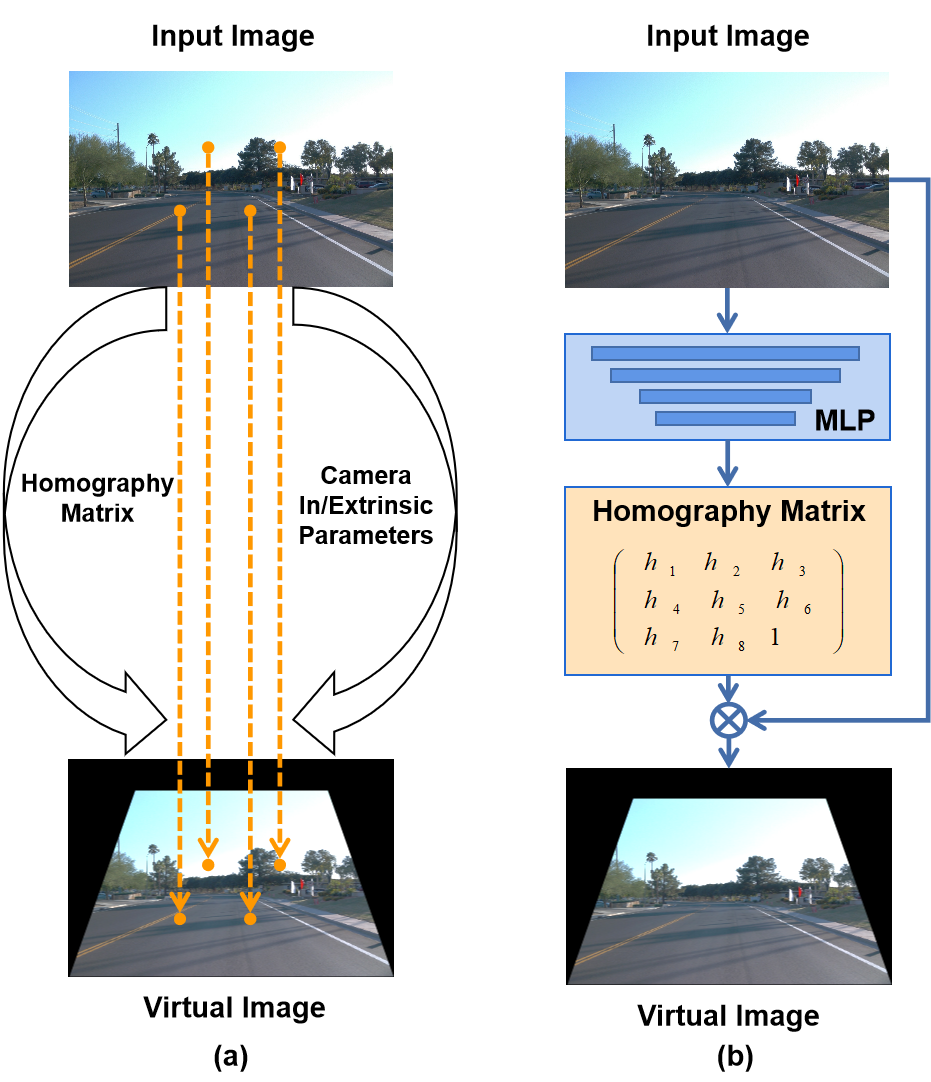
\includegraphics[width=0.8\linewidth]{asset/fvhnet}
    \caption{(a) Fixed parameters transformation matrix, which based on camera in/external parameters.
        (b) MLP-based transformation matrix, which learns a perspective transformation conditioned on the input image.}
    \label{fig:intro}
\end{figure}

Among these methods for 3D lane line detection, BEV-based methods~\cite{chen2022persformer, efrat20203d, guo2020gen, liu2022learning, wang2023bev} have received attention from researchers due to the accuracy, robustness, and speed.
These methods need a spatial transformation module to transform front-view features to bev-view.
In Bev-LaneDet\cite{wang2023bev}, spatial transformation module is fixed spatial mapping by MLP,
which are difficult to be integrated with the camera in/extrinsic parameters, resulting in poor performance.
To address this issue, it realizes a preprocessing method of quickly
unifying the camera in/extrinsic parameters by establishing
a Virtual Camera with standard in/extrinsic parameters, which are fixed parameters derived from the mean value of the in/extrinsic
parameters of the training dataset.
However, different cameras mounted on the vehicle have different internal/external parameters, which have a significant effect on features transformation and 3D lane results.
As illustrated in Fig.\ref{fig:intro}(a)\@, if a fixed transformation matrix is employed to get homography matrix for features transformation, the projection becomes less accurate.
Therefore, we need unify the in/extrinsic parameters of front-facing cameras on different vehicles.

Towards this issue, we proposed a MLP-based homography matrix estimation network,
called \textbf{F}ront-\textbf{V}irtual \textbf{H}omograph Matrix Net, which makes homography matrix learnable instead of fixed.
As show in Fig.\ref{fig:intro}(b)\@. FVHNet takes the RGB image as input and predicts the parameters to generate the homography matrix.
We project the input images to the virtual camera by multiplying the homography matrix.
After this transformation, we input the virtual-view image features to backbone network which output the front-view features.
Then, we can get the 2d prediction by a front-view lane detection head.
Finally, the front-view prediction is re-projected back to the original image space by multiplying the inverse homography matrix
and compute the loss between the prediction and ground truth.
Through this way, the model can be trained effectively without providing any extra annotations except for the original lane labels.


\textbf{In general, our main contributions are three-fold:}
% hzm----
%\textbf{1)} We propose to extract homographic parameters from input image by MLP networks, making homography matrix learnable.
%With a more accurate homographic matrix, in/extrinsic can be unified in a more robust virtual camera. We propose to extract homographic parameters from input image by MLP networks, making homography matrix learnable.
\textbf{1)} FVHNet, a MLP-based network that can learn transformation matrix parameters which can transform input images to virtual camera images.
\textbf{2)} FVHLoss, a loss function to supervise FVHNet training, which only needs the annotations of lane marks.
%\textbf{3)} We conducted experiments on both real and synthetic datasets, This method shows remarkable detection accuracy on both the OpenLane and Apollo Synthetic datasets;
\textbf{3)} Our method is validated on the Apollo 3D synthetic dataset, achieving the promising performance. %compared with

%\let\thefootnote\relax\footnotetext{\footnoterule This work is supported by Beijing Natural Science Foundation (L221011).}
%\vspace*{\fill} % 将acknowledgement置于页面底部
%\footnoterule % 分隔线
%\footnotesize
%\noindent \textbf{Acknowledgement:} This work is supported by Beijing Natural Science Foundation (L221011).
%\noindent *Corresponding author

%%%%%%%%% RELATED_WORK
\section{Related Work}
\label{sec:relatedwork}

\subsection{2D Lane Detection}
\label{subsec:2d}
%anchor3d

2D lane detection~\cite{chen2023improving, jin2022eigenlanes, liu2021end, pan2018spatial, tabelini2021polylanenet, yang2023lane}
aims at obtaining the accurate shape and locations of lanes in the images, which is not concerned with the spatial extension of the lane line.
Earlier works~\cite{aly2008real, he2004color, kim2008robust, wang2004lane, zhou2010novel, srivastava2014improved, chanawangsa2012new}
mainly focus on extracting low-level handcrafted features, such as edge and color information.
However, these approaches are less robust under changing scenarios and often have complex feature extraction and post-processing designs.
Benefiting from deep learning, 2D lane detection has made significant progress.
These works are divided into four categories according to segmentation-based methods, keypoint-based methods, curve-based parameters, anchor-based methods.

\textbf{Segmentation-based methods}~\cite{hou2019learning, neven2018towards, pan2018spatial, qin2020ultra, dong2023hybrid, lee2023end}
formulate 2D lane detection task as a pixel-wise classification problem, which the computing cost is expensive.

\textbf{Keypoint-based methods}~\cite{ko2021key, qu2021focus, wang2022keypoint, xu2022rclane}
focus on identifying and localizing specific key points or landmarks along lane boundaries in images or videos.
These methods aim to simplify the lane detection process by directly detecting key features of the lanes.
While keypoint-based methods can be efficient, they may face challenges in scenarios where key points are not well-defined or when there is significant noise or clutter in the image.
Additionally, accurately identifying key points in varying environmental conditions can be a demanding task.

\textbf{Curve-based methods}~\cite{feng2022rethinking, tabelini2021polylanenet, chen2023improving} focus on identifying and characterizing lane boundaries using mathematical curve representations.
These methods aim to model the lanes as curves, such as quadratic or cubic functions, and estimate the parameters of these curves to accurately detect and localize the lanes.
These works proposed that the 2D lane detection can be converted into the problem of curve parameter regression by detecting the starting point, ending point, and curve parameters.

\textbf{anchor-based methods}~\cite{li2019line, liu2021condlanenet, tabelini2021keep, zheng2022clrnet, ran2023flamnet, huang2023anchor3dlane} design line-like anchors and estimate the offsets between sampled points and predefined anchor points, making them particularly suitable for scenarios with distinct lane patterns.
Non-Maximum Suppression (NMS) is then employed to select the lane lines with the highest confidence.
LineCNN~\cite{li2019line} first defines straight rays emitted from the image boundary to fit the shape of 2D lane lines and applies Non-Maximum Suppression (NMS) to keep only lanes with higher confidence.
LaneATT~\cite{tabelini2021keep} proposes an anchor-based pooling method and an attention mechanism to aggregate more global information.
CLRNet~\cite{zheng2022clrnet} learns to refine the initial anchors iteratively through the feature pyramid.

\subsection{3D Lane Detection}
\label{subsec:3d}
Since projecting 2D lanes into 3D space suffers from inaccuracy as well as less robustness, many researchers have turned their attention to lane detection in 3D space.
Unlike traditional 2D methods that operate solely in the image plane, 3D lane detection leverages depth information to provide a more comprehensive understanding of the road environment,
enabling vehicles to perceive and navigate lanes in real-world scenarios with varying terrains, elevation changes, and complex road geometries.

Some works restore 3D information using multiple sensor~\cite{cordts2016cityscapes, luo2022m, chen2022persformer}.
While 3D lane detection offers significant advantages, it also comes with challenges such as computational complexity,
sensor calibration and the collection and annotation cost of multisensor data is expensive.
Therefore, monocular camera image based 3D lane detection~\cite{efrat20203d, garnett20193d, guo2020gen, liu2022learning, yan2022once, huang2023anchor3dlane, wang2023bev} attracts more attention.

Due to the good geometric properties of lanes in the perspective of BEV, \textbf{3DLaneNet}~\cite{garnett20193d} predict the position of lanes in 3D space.
It utilizes an Inverse Perspective Mapping (IPM) technique to transform features from a front-view image into a Bird's Eye View (BEV) representation,
where the geometric properties of lanes are more easily discernible.
By regressing the anchor offsets in the BEV space, 3DLaneNet can accurately predict the position of lanes without relying on the assumption of a flat ground.
\textbf{Gen-LaneNet}~\cite{guo2020gen} improves the alignment between the virtual top view generated by an inverse perspective mapping (IPM) and the true top view in 3D space.
By distinguishing between these views, Gen-LaneNet enhances the accuracy of lane detection without the need for a bird's-eye view (BEV) transformation.
\textbf{Persformer}~\cite{chen2022persformer} utilizes deformable attention to generate bird's-eye-view (BEV) features more adaptively and robustly, improving the accuracy and reliability of 3D lane detection without relying on the flat ground assumption.
\textbf{SALAD}~\cite{yan2022once} tries to get rid of BEV by decomposing 3D lane detection into 2D lane segmentation and dense depth estimation tasks.
\textbf{Anchor3DLane}~\cite{huang2023anchor3dlane} predict 3D lanes directly from frontal-viewed (FV), which defines 3D lane anchors in the 3D space and projects them onto the FV features to extract structural and contextual information for accurate predictions, and incorporates a global optimization technique to reduce lateral prediction errors by leveraging the equal-width property between lanes.
\textbf{BEV-LaneDet}~\cite{wang2023bev} establishes a Virtual Camera with standard in/extrinsic parameters to ensure the consistency in the spatial relationship among cameras, and introduces a Spatial Transformation Pyramid module for transforming front-view features into Bird's Eye View (BEV) features.

%%%%%%%%% METHODS

\begin{figure*}[ht]
    \centering
    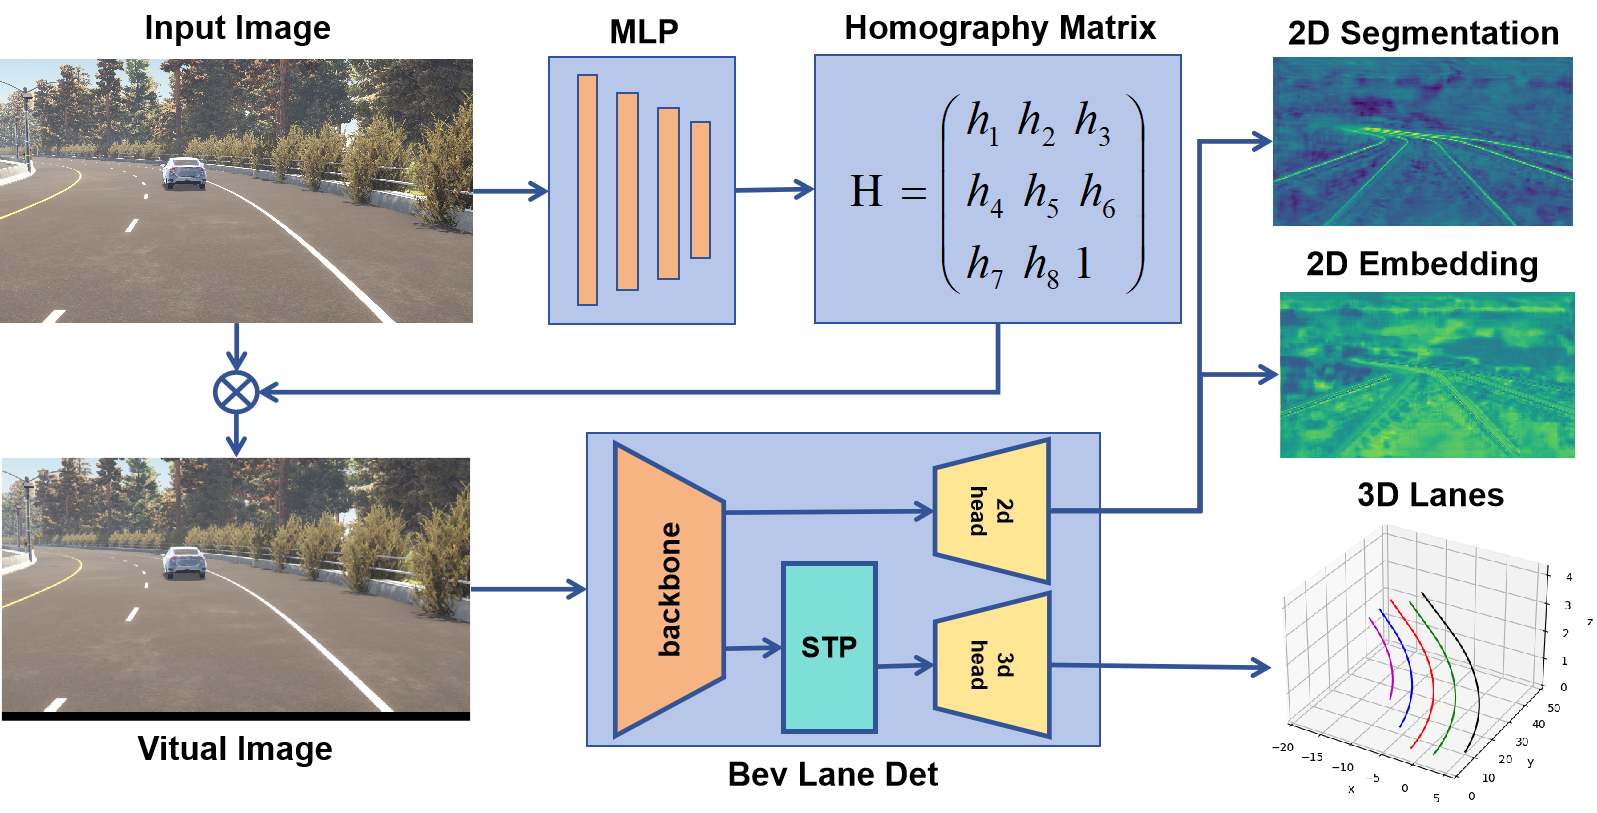
\includegraphics[height=0.45\textheight]{asset/structure} %width=1\linewidth
    \caption{Overview of the framework}
    \label{fig:overview}
\end{figure*}

\section{Methods}
\label{sec:methods}
%Fig.\ref{fig:overview} shows the overview of our entire lane detection framework.
An overview of our entire lane detection framework is illustrated in Fig.\ref{fig:overview}.
Our approach takes a single image captured by a front camera mounted on the vehicle as input information.
The image from the current camera is projected onto the view of the virtual camera using the homography
matrix generated by MLP network \cite{tang2022image},
which aims to transform the in/external parameters of the input image to a unified
in/external parameter of the virtual camera.
We use ResNet18 and ResNet34 \cite{he2016deep} as our backbone to extract front view image features.
Spatial Transformation Pyramid \cite{wang2023bev} transform the front view features into BEV features.
Then, lanes are predicted on the BEV view. We predict the confidence of each cell, the embedding used for clustering,
the offset from the center of the cell to the lane in the y-direction, and the height.
we added the front view lane detection header as an
auxiliary supervision to improve backbone's ability to extract front view features
and supervise the homography matrix estimation network's training.

\subsection{Homography}
new
why use homography?
If a fixed transformation matrix is employed, the projection becomes less accurate when sloping ground planes or camera vibrations are encountered.
To remedy this situation, we train a network to output certain crucial parameters in the perspective transformation.

101
011
001
A full projection model describes the mapping from world to pixel coordinates.
For this nonlinear projection, more unknown model parameters mean a higher risk of unstable output.
Fully constructing a 3 × 3 homographic matrix needs 8 dependent components.
However, treating each of them as an independent parameter is not a good idea since they are actually correlated.
Therefore, we set up a homographic model from the fundamental projection principle and try to reduce the number of outputs to the least degrees of freedom in H.
Depending on whether the camera is pre-calibrated, different outputs of the model are designed.

The zeros are placed to enforce the constraint that horizontal lines remain horizontal under the transformation.

old
A homography is a projective transformation between two planes or, alternatively, a mapping between two planar projections of an image.
In other words, homographies are simple image transformations that describe the relative motion between two images, when the camera (or the observed object) moves.
It is the simplest kind of transformation that describes the 2D relationship between two images.
Homography can be mathematically described by a 3D transformation in a homogeneous coordinates space and can be expressed as:

\[
S\left[ \begin{matrix}
   x'  \\
   y'  \\
   1
\end{matrix} \right]
=
H\left[ \begin{matrix}
   x  \\
   y  \\
   1
\end{matrix} \right]
=
\left[ \begin{matrix}
h_1 & h_2 & h_3  \\
h_4 & h_5 & h_6  \\
h_7 & h_8 & h_9  \\
\end{matrix} \right]
\left[ \begin{matrix}
x  \\
y  \\
1
\end{matrix} \right]
\]
where H denotes the homography matrix $H \in R^{3\times 3}$ between two two-dimensional planes,
which allows us to switch from one view of the same scene to another by multiplying
the homography matrix with the points [u,v] in one view to find their corresponding positions [u',v'] in the other view.
The homography matrix is usually parameterized by the elements of a 3×3 matrix,
but it has only 8 degrees of freedom, and a simple way to do this is to hardcode $h_9=1$.
We take the original image as input and use DNN to estimate eight parameters of the homography matrix.


\begin{figure}[!ht]
    \centering
    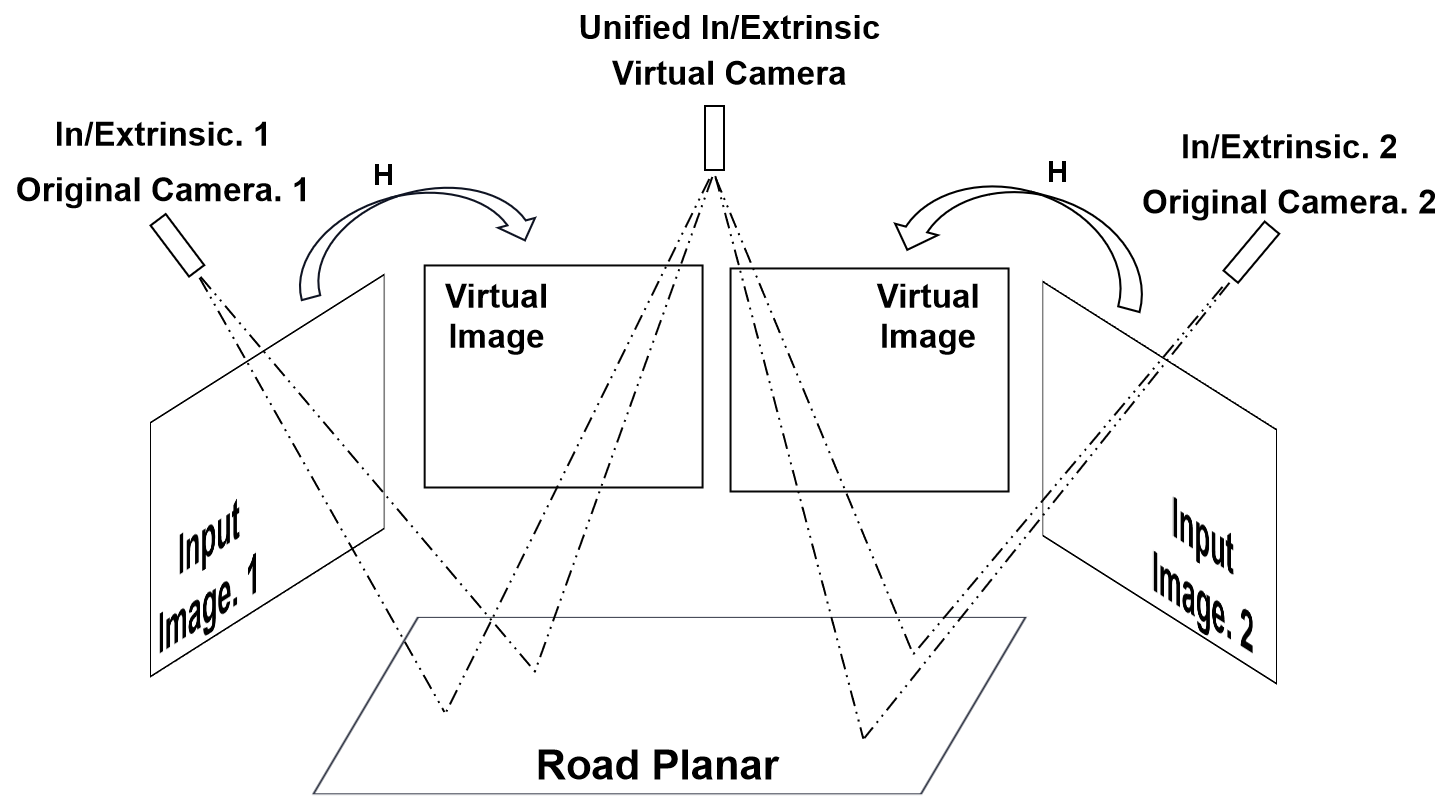
\includegraphics[width=\linewidth]{asset/virtual_camera}
    \caption{Virtual Camera}
    \label{fig:Virtual Camera}
\end{figure}

\begin{figure*}[!ht]
    \centering
    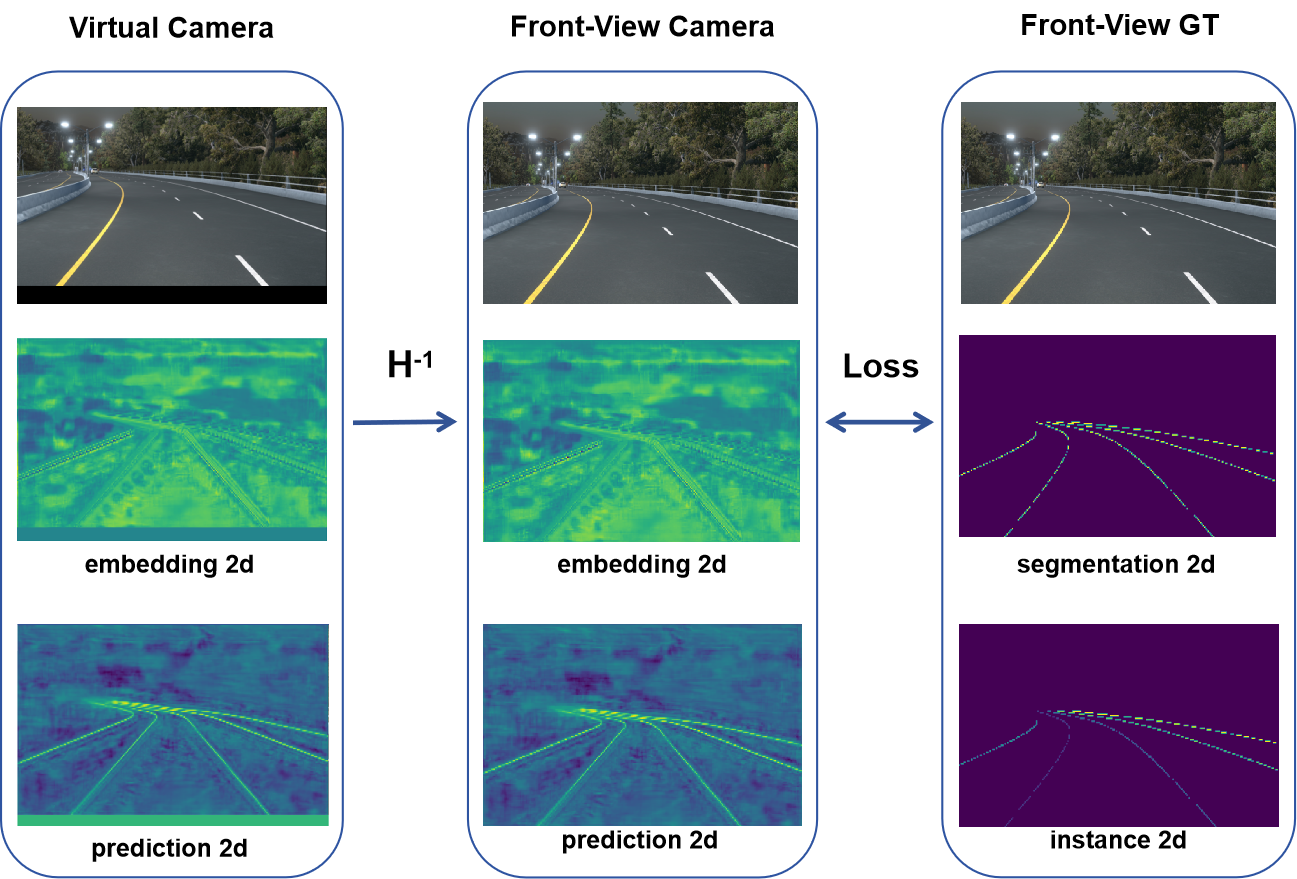
\includegraphics[height=0.45\textheight]{asset/loss2}
    \caption{Homography Loss}
    \label{fig:Homography Loss}
\end{figure*}

\subsection{Unified Camera Parameters}
\label{subsec:Unified Camera Parameters}
Different cameras mounted on the vehicle have different internal/external parameters,
which have a significant effect on the 3D lane results.
As shown in Fig.\ref{fig:Virtual Camera},
By creating a virtual camera with standard internal/external parameters,
we can unify the internal/external parameters of different cameras.
We project the image of the current camera into the view of the virtual camera through the homography matrix H based on the principle of perspective transformation.
As a result, the virtual camera unifies the internal/external parameters of different cameras.
%Wave-MLP  \cite{tang2022image} represents each token as a wave function with two parts,
%amplitude and phase, which can model different contents from different input images.
We use a MLP network to estimate the 8 parameters of the homography matrix from the input frames.
Then, we transform from one view of the same scene to another by multiplying the homography matrix with the points $[u,v]$ in one view
to find their corresponding locations $[u',v']$ in the other view.

\subsection{Homography Loss}
\label{subsec:Homography Loss}
as shown in Fig.\ref{fig:Homography Loss}. In order to improve the MLP network's ability to extract homography matrix parameters and backbone's ability to extract front view features,
a front view lane detection header was added as an auxiliary supervision.
Based on this front view lane detection head, we propose the homography loss function.
After the input image is converted to a virtual camera image by homography matrix $H$,
the front view features of the virtual camera image are obtained by backbone,
and the front view lane detection head gets the virtual camera segmentation and embedding results ${Seg}_{v}, {Emb}_{v}$,
which can be converted back to the input camera ${Seg}_{i}, {Emb}_{i}$ by the inverse matrix $H^{-1}$ of the homography matrix.
The front-view lane loss includes lane segmentation loss and lane embedding loss, referred to LaneNet \cite{neven2018towards}.The homography loss is defined as follows,
\[
L_{h}=\lambda_{seg}^h L_{seg}^h + \lambda_{emb}^h L_{emb}^h
\]
where $L_{seg}^h$ denotes lane segmentation loss, and$L_{emb}^h$ denotes lane embedding loss in the front-view.


%%%%%%%%% EXPRIMENTS
\section{Expriments}

\begin{table*}[!ht]
    \caption{Comparison with previous methods on Apollo 3D Lane Synthetic Dataset.}\label{tab:table1}
    \center
%    \resizebox{1\linewidth}{!}{ % 表格环境外部设置(头)
    \begin{tabular}{ccccccc}% 其中,tabular是表格内容的环境;c表示centering,即文本格式居中;c的个数代表列的个数
        \toprule %[2pt]设置线宽
        Scene Method & F-Score & X error near & X error far & Z error near & Z error far \\
        \toprule %[2pt]设置线宽
        \multirow{2}{*}{Balanced Scence} & 3D-LaneNet [8] & 86.4 & 0.068 & 0.477 & 0.015 & \textbf{0.202} \\ %换行
        \multirow{2}{*}{ }               & Gen-LaneNet [9] & 88.1 & 0.061 & 0.496 & 0.012 & 0.214  \\
        \multirow{2}{*}{ }               & 3D-LaneNet(1/att) [13] & 91 & 0.082 & 0.439 & 0.011 & 0.242  \\
        \multirow{2}{*}{ }               & Gen-LaneNet(1/att) [13] & 90.3 & 0.08 & 0.473 & 0.011 & 0.247  \\
        %\multirow{2}{*}{ }               & CLGO [19] & 91.9 & 0.061 & 0.361 & 0.029 & 0.25  \\
        %\multirow{2}{*}{ }               & Reconstruct from Top [14] & 91.9 & 0.049 & 0.387 & \textbf{0.008} & 0.213  \\
        \multirow{2}{*}{ }               & PersFormer [3] & 92.9 & 0.054 & 0.356 & 0.01  & 0.234 \\
        \multirow{2}{*}{ }               & Ours       & \textbf{97.2} & \textbf{0.033} & \textbf{0.273} & 0.044 & 0.263 \\
        \midrule %[2pt]
        \multirow{2}{*}{Rarely Observed} & 3D-LaneNet [8] & 72 & 0.166 & 0.855 & 0.039 & \textbf{0.521} \\
        \multirow{2}{*}{ }               & Gen-LaneNet [9] & 78 & 0.139 & 0.903 & 0.03 & 0.539  \\
        \multirow{2}{*}{ }               & 3D-LaneNet(1/att) [13] & 84.1 & 0.289 & 0.925 & 0.025 & 0.625  \\
        \multirow{2}{*}{ }               & Gen-LaneNet(1/att) [13] & 81.7 & 0.283 & 0.915 & 0.028 & 0.653  \\
        %\multirow{2}{*}{ }               & CLGo [19] & 86.1 & 0.147 & 0.735 & 0.071 & 0.609  \\
        %\multirow{2}{*}{ }               & Reconstruct from Top [14] & 83.7 & 0.126 & 0.903 & \textbf{0.023} & 0.625  \\
        \multirow{2}{*}{ }               & PersFormer [3] & 87.5 & 0.107 & 0.782 & 0.024 & 0.602 \\
        \multirow{2}{*}{ }               & Ours       & \textbf{95.5} & \textbf{0.059} & \textbf{0.646} & 0.090 & 0.685 \\
        \midrule %[2pt]
        \multirow{2}{*}{Vivual Variants} & 3D-LaneNet [8] & 72.5 & 0.115 & 0.601 & 0.032 & \textbf{0.23}  \\
        \multirow{2}{*}{ }               & Gen-LaneNet [9] & 85.3 & 0.074 & 0.538 & 0.015 & 0.232  \\
        \multirow{2}{*}{ }               & 3D-laneNet(1/att) [13] & 85.4 & 0.118 & 0.559 & 0.018 & 0.29  \\
        \multirow{2}{*}{ }               & Gen-LaneNet(1/att) [13] & 86.8 & 0.104 & 0.544 & 0.016 & 0.294  \\
        %\multirow{2}{*}{ }               & CLGo [19]  & 87.3  & 0.084  & 0.464  & 0.045  & 0.312  \\
       % \multirow{2}{*}{ }               & Reconstruct from Top [14]  & 89.9  & 0.06  & 0.446  & \textbf{0.011}  & 0.235  \\
        \multirow{2}{*}{ }               & PersFormer [3] & 89.6 & 0.074 & 0.43  & 0.015 & 0.266 \\
        \multirow{2}{*}{ }               & Ours       & \textbf{94.3} &\textbf{ 0.051} & \textbf{0.389} & 0.043 & 0.307 \\
        \bottomrule %[2pt]
    \end{tabular}
%    }% 外部环境设置(尾)
\end{table*}

\subsection{Dataset And Experimental Setup}
\label{subsec:Dataset And Experimental Setup}
%OpenLane contains 150,000 training frames and 40,000 test frames.
%In order to verify the performance of the model for every scene, the Up\&Down case, Curve case, Extreme Weather case,
%Intersection case, Merge\&Split case, and Night case are separated from the validation set.

\textbf {apollo 3D Lane Synthetic Dataset}. Apollo Synthetic
dataset \cite{guo2020gen} consists of over 10k 1080 × 1920 images which
are built using unity 3D engine, including highway, urban,
residential and downtown environments. The dataset is split
into three different scenes: balanced scenes, rarely observed
scenes and scenes with visual variations for evaluating algorithms from different perspectives.

\textbf {OpenLane Dataset}. OpenLane Dataset \cite{chen2022persformer} is the first
real world 3D lane dataset which consists of over 200K
frames at a frequency of 10 FPS based on Waymo Open
dataset [32], [33]. In total, it has a training set with 157k
images and a validation set of 39k images. The dataset
provides camera intrisics and extrinsics following the same
data format as Waymo Open Dataset.


\subsection{Experiment Settings}
\label{subsec:Experiment Settings}
Implementation Details. We use ResNet \cite{he2016deep} as backbone.
The resolution of our input image is 576 × 1024.
The bev range is set to [3, 103] × [-12, 12] along x and y respectively.
Each cell represents x × x (x defaults to 0.5m).
Our network uses Adam optimizer \cite{kingma2014adam}, with a base learning rate of $10^{-3}$ and weight decay of $10^{-2}$.
All models are trained from scratch with 120 epochs and the per-GPU batch size is set to 8.

\subsection{Evaluation}
\label{subsec:Evaluation}
The evaluation metrics we used are referred from Gen-LaneNet \cite{guo2020gen}, which includes F-Score in different scenes and X/Z error in different regions.
We report Average Precision (AP) , Fscore, and errors (near range and far range) to investigate the performance of our model.

\subsection{Comparisons with existing methods}


%%%%%%%%% CONCLUSIONS
\section{Conclusions}
conclusion 
conclusion 
conclusion
%-------------------------------------------------------------------------

%%%%%%%%% ACKNOWLEDGEMENT
%\section{Acknowledgement}
This work is supported by Beijing Natural Science Foundation (L221011).
%-------------------------------------------------------------------------

%%%%%%%%% REFERENCES
%\clearpage
\bibliography{IEEEtran/NameofReference}

%-------------------------------------------------------------------------
%%%%%%%%% APPENDIX
%\appendix
\section{Appendix}

appendix
appendix
appendix
appendix

\end{document}
